\documentclass[aspectratio=169, 10pt]{ctexbeamer}

%--- Packages ---
\usepackage{amsmath, amssymb, amsthm}
\usepackage{bm}
\usepackage{graphicx}
\usepackage{booktabs}
\usepackage{listings}
\usepackage{xcolor}
\usepackage{tikz}
\usepackage{hyperref}
\usepackage{caption}

%--- Theme Settings ---
\usetheme{Madrid}
\usecolortheme{dolphin}
\usefonttheme{professionalfonts}

%--- Image Path Configuration ---
% 设置图片搜索路径,以应对不同的文件存放结构
\graphicspath{{/home/ztc2025/plyproj/wvp/essay/picture/}}

%--- Colors for Code ---
\definecolor{codegreen}{rgb}{0,0.6,0}
\definecolor{codegray}{rgb}{0.5,0.5,0.5}
\definecolor{codepurple}{rgb}{0.58,0,0.82}
\definecolor{backcolour}{rgb}{0.95,0.95,0.92}

\lstdefinestyle{mystyle}{
    backgroundcolor=\color{backcolour},   
    commentstyle=\color{codegreen},
    keywordstyle=\color{magenta},
    numberstyle=\tiny\color{codegray},
    stringstyle=\color{codepurple},
    basicstyle=\ttfamily\footnotesize,
    breakatwhitespace=false,         
    breaklines=true,                 
    captionpos=b,                    
    keepspaces=true,                 
    numbers=left,                    
    numbersep=5pt,                  
    showspaces=false,                
    showstringspaces=false,
    showtabs=false,                  
    tabsize=2
}
\lstset{style=mystyle}

%--- Citation Helper ---
\newcommand{\mycite}[1]{\let\thefootnote\relax\footnotetext{\tiny \textcolor{gray}{[Ref] #1}}}

%--- Title Info ---
\title[FALQON Zero-Shot Inference]{基于 Transformer 架构与谱嵌入的\\反馈诱导量子优化算法(FALQON)参数零次推理}

\author[潘立扬]{潘立扬}

\date{\today}

\begin{document}

%--- Title Page ---
\begin{frame}
    \titlepage
\end{frame}

%--- Outline ---
%\begin{frame}{目录}
 %   \tableofcontents
%\end{frame}

%===========================================================
\section{研究背景与动机}
%===========================================================

\begin{frame}{研究背景与动机}
    \begin{columns}
        \column{0.55\textwidth}
        \textbf{1. NISQ 时代的挑战: 变分参数优化}
        \begin{itemize}
            \item \textbf{QAOA 困境}: 经典优化循环需要在高维非凸景观中搜索参数 $\bm{\theta}^*$,面临局部极小值与\textbf{贫瘠高原 (Barren Plateaus)} 问题。
        \end{itemize}

        \vspace{0.5em}
        \textbf{2. 现有解法: FALQON (Magann et al.)}
        \begin{itemize}
            \item \textbf{机制}: 基于量子李雅普诺夫控制 (QLC) 的确定性反馈律。
            \item \textbf{优势}: 理论保证能量 $E_p$ 随深度 $p$ 单调递减,\textbf{无需}外部经典优化器。
        \end{itemize}

        \vspace{0.5em}
        \textbf{3. 新的瓶颈: 测量开销 (Measurement Overhead)}
        \begin{itemize}
            \item \textbf{问题}: 反馈律依赖对易子期望 $\langle i[H_d, H_p] \rangle$。
            \item \textbf{代价}: 每增加一层都要在量子硬件上进行大量重复测量 (Shots),且需抵抗 Shot Noise,导致\textbf{执行效率低}。
        \end{itemize}

        \column{0.45\textwidth}
        \begin{alertblock}{本文方案: Teacher-Student 零次推理}
            \begin{itemize}
                \item \textbf{Teacher}: 经典仿真运行 FALQON 产生轨迹。
                \item \textbf{Student}: Transformer 学习 $G \to \{\beta_p\}$ 的非线性映射。
                \item \textbf{Outcome}: \textbf{消除}在线反馈测量,毫秒级生成参数。
            \end{itemize}
        \end{alertblock}
    \end{columns}
    
    \mycite{[3] Magann et al., Phys. Rev. Lett. (2022); [6,7] QAOA-GPT \& Transferability}
\end{frame}

\begin{frame}{核心方案对比:突破测量瓶颈}
    \begin{figure}
        \centering
        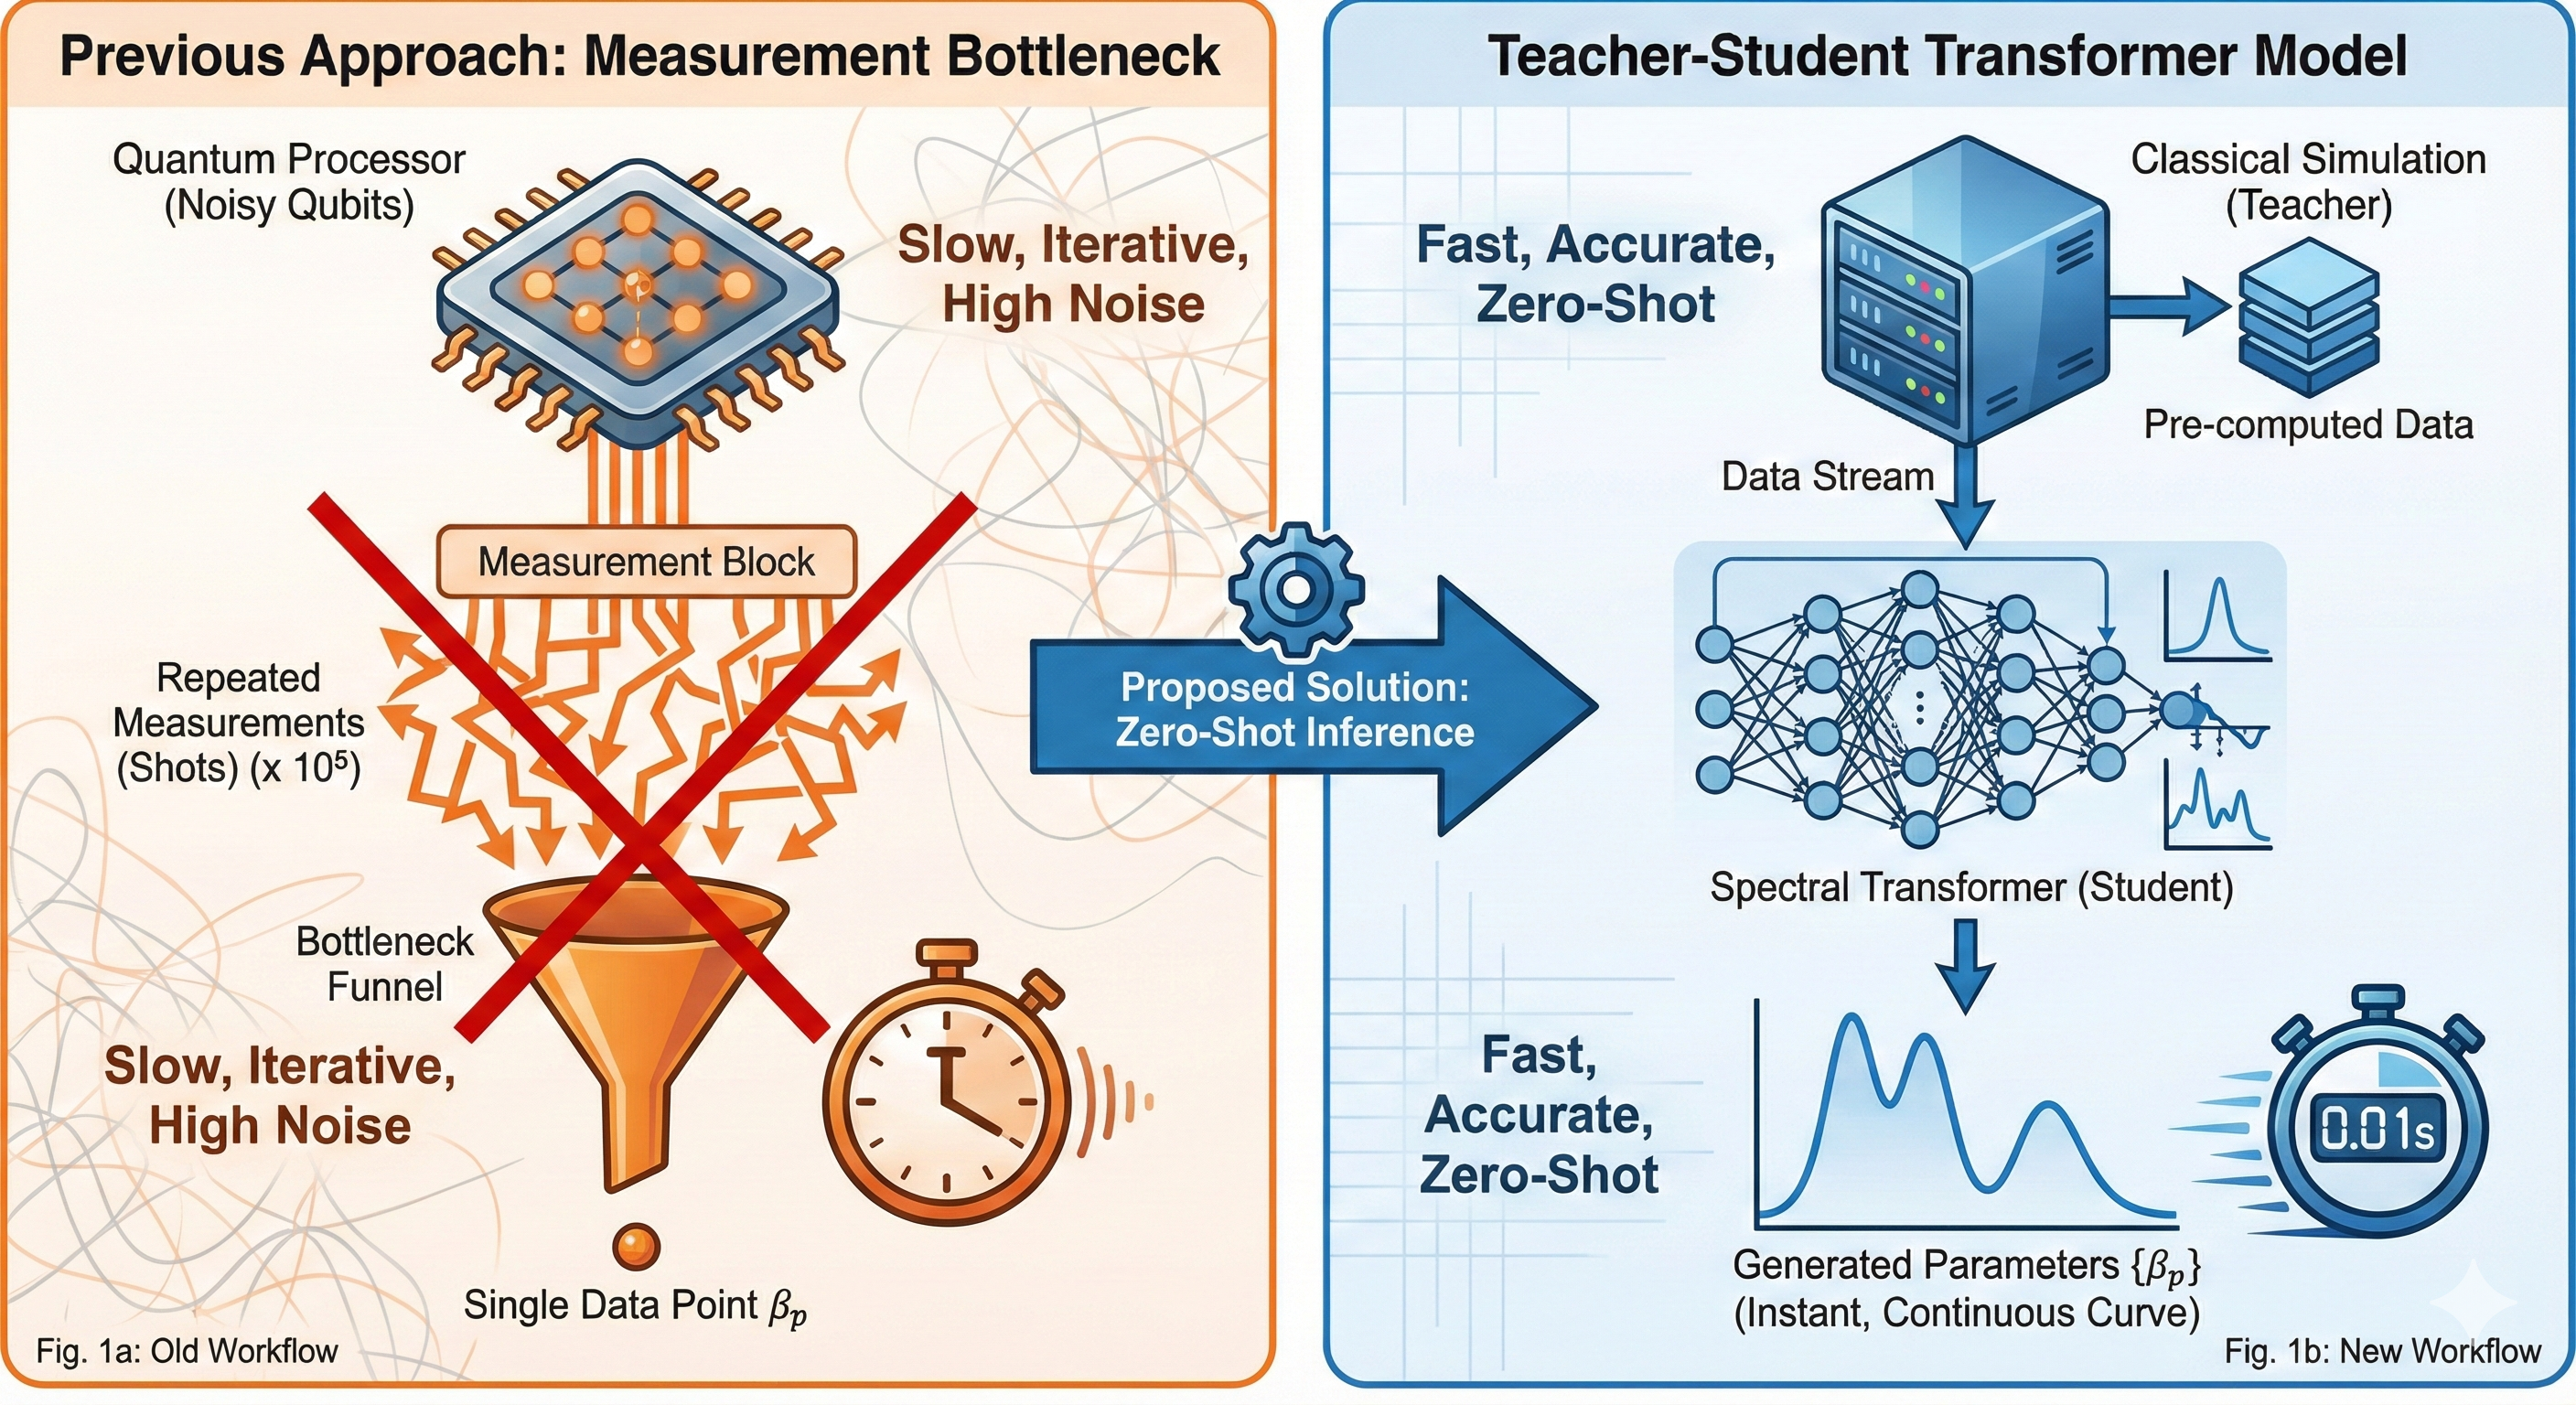
\includegraphics[width=0.75\textwidth]{workflow_comparison.png}
        \caption{传统 FALQON (左) 与本文 Teacher-Student 零次推理框架 (右) 的工作流对比。新架构通过离线学习 Teacher 轨迹,实现了对 $p$ 层参数的瞬时预测,消除了在线闭环测量带来的巨大时间开销。}
    \end{figure}
\end{frame}

%===========================================================
\section{理论方法与公式}
%===========================================================


\begin{frame}{FALQON 动力学机制}
    考虑由问题哈密顿量 $H_p$ 和驱动哈密顿量 $H_d$ 描述的系统。目标是最小化成本函数 $C(t)=\langle\psi(t)|H_p|\psi(t)\rangle$。根据薛定谔方程,其对时间的导数为:
\begin{equation}
\frac{d C(t)}{dt} = i \beta(t) \langle \psi(t) | [H_d, H_p] | \psi(t) \rangle.
\end{equation}
为了确保成本函数随时间单调递减(即 $dC/dt\le 0$),构造反馈控制律:
\begin{equation}
\beta(t) = -\alpha\,\langle \psi(t) | i[H_d, H_p] | \psi(t) \rangle.
\end{equation}
在 FALQON 的离散化实现中,状态演化算符为 $U_p=e^{-i\beta_p H_d}e^{-iH_p\Delta t}$。

项目实现中首先预计算 $A=i(H_d H_p - H_p H_d)$(见算法文件),并在每层更新
\[
\beta_p = -\alpha\,\langle \psi_p|A|\psi_p\rangle,\quad \psi_{p+1}=e^{-i\beta_p H_d}e^{-iH_p}\,\psi_p.
\]

这使得我们可以把“反馈生成的 $\beta$ 序列”看作一个监督信号,用于训练学生模型回归整段轨迹。

\end{frame}

\begin{frame}{FALQON 动力学机制}
    \textbf{定理(FALQON 收敛性):}
定义李雅普诺夫函数 $V(\boldsymbol{\beta}) = \langle \psi(\boldsymbol{\beta}) | H_P | \psi(\boldsymbol{\beta}) \rangle$。
根据薛定谔方程 $i\frac{\partial}{\partial t}|\psi\rangle = H(t)|\psi\rangle$,其中 $H(t) = H_P + \beta(t)H_d$(设 $\hbar=1$),我们有目标函数的导数:
\begin{equation}
\frac{d}{dt}\langle H_P \rangle = i \langle \psi | [H(t), H_P] | \psi \rangle = i \beta(t) \langle \psi | [H_d, H_P] | \psi \rangle
\end{equation}
设定反馈律 $\beta(t) = -\alpha \cdot i \langle [H_d, H_P] \rangle$(其中 $\alpha > 0$),由于 $H_d, H_P$ 均为厄米算符,其对易子的期望值为纯虚数,故 $i \langle [H_d, H_P] \rangle$ 为实数。代入后得:
\begin{equation}
\frac{d}{dt}\langle H_P \rangle = - \alpha \left( i \langle [H_d, H_P] \rangle \right)^2 \le 0
\end{equation}
这保证了能量随演化时间单调非递增,即系统必然流向 $H_P$ 的低能子空间。


\end{frame}




\begin{frame}{收敛性与鲁棒性}

    \textbf{收敛性:} 由FALQON 收敛性给出

    \begin{equation}
        \frac{dV}{dt} = -\alpha \left( \langle i[H_p, H_c] \rangle \right)^2 \le 0
    \end{equation}

    \vspace{0.5em}
    
    \textbf{对预测误差的鲁棒性}:
    \begin{itemize}
        \item 学生模型预测 $\tilde{\beta} = \beta_{\text{teacher}} + \epsilon$。
        \item 只要 \textcolor{blue}{$\text{sgn}(\tilde{\beta}) = \text{sgn}(\beta_{\text{teacher}})$},则 $\frac{dV}{dt}$ 依然非正。
        \item \textbf{结论}: FALQON 对\textbf{幅度误差}不敏感,但对\textbf{符号误差}敏感。这解释了为何 MSE 非零时 AR 依然很高,同时也凸显了 SignNet 解决符号歧义的重要性。
    \end{itemize}

    \mycite{[2, 5, 13] Robust Feedback-Based Quantum Optimization}
\end{frame}

\begin{frame}{图结构的哈密顿量编码}

\begin{equation}
H_p = \sum_{(i,j) \in E} w_{ij} \frac{I - Z_i Z_j}{2}.
\end{equation}
由于 $H_p$ 完全由图的邻接矩阵 $A$ 决定,参数轨迹 $\vec{\beta}$ 是矩阵 $A$ 的非线性函数。本文假设存在映射 $\mathcal{F}:A\mapsto\vec{\beta}$,并利用神经网络进行逼近。

\textbf{Cut 与能量的换算:} 在代码评估中,我们以能量期望 $E=\langle H_p\rangle$ 换算切割值:
\begin{equation}
\mathrm{Cut} = \frac{|E(G)| - 2E}{2},\qquad \mathrm{AR}=\frac{\mathrm{Cut}_{\mathrm{AI}}}{\mathrm{Cut}_{\mathrm{FALQON}}}.
\end{equation}

\end{frame}



\begin{frame}{模型架构:Spectral Embedding + Transformer}
    \begin{columns}
        \column{0.4\textwidth}
        为了处理图数据的置换不变性,我们采用了谱嵌入 (Spectral Embedding) 作为输入特征。
        
        \begin{itemize}
            \item \textbf{输入特征}: 拉普拉斯矩阵 $L$ 的特征分解 $\Lambda, V$。
            \item \textbf{SignNet}: 解决特征向量的符号模糊性 $\rho(\sum \phi(v_i))$。
            \item \textbf{Transformer}: 捕捉全局依赖。
        \end{itemize}
        \mycite{Lim et al., ICLR (2023)}

        \column{0.6\textwidth}
        \begin{figure}
            \centering
            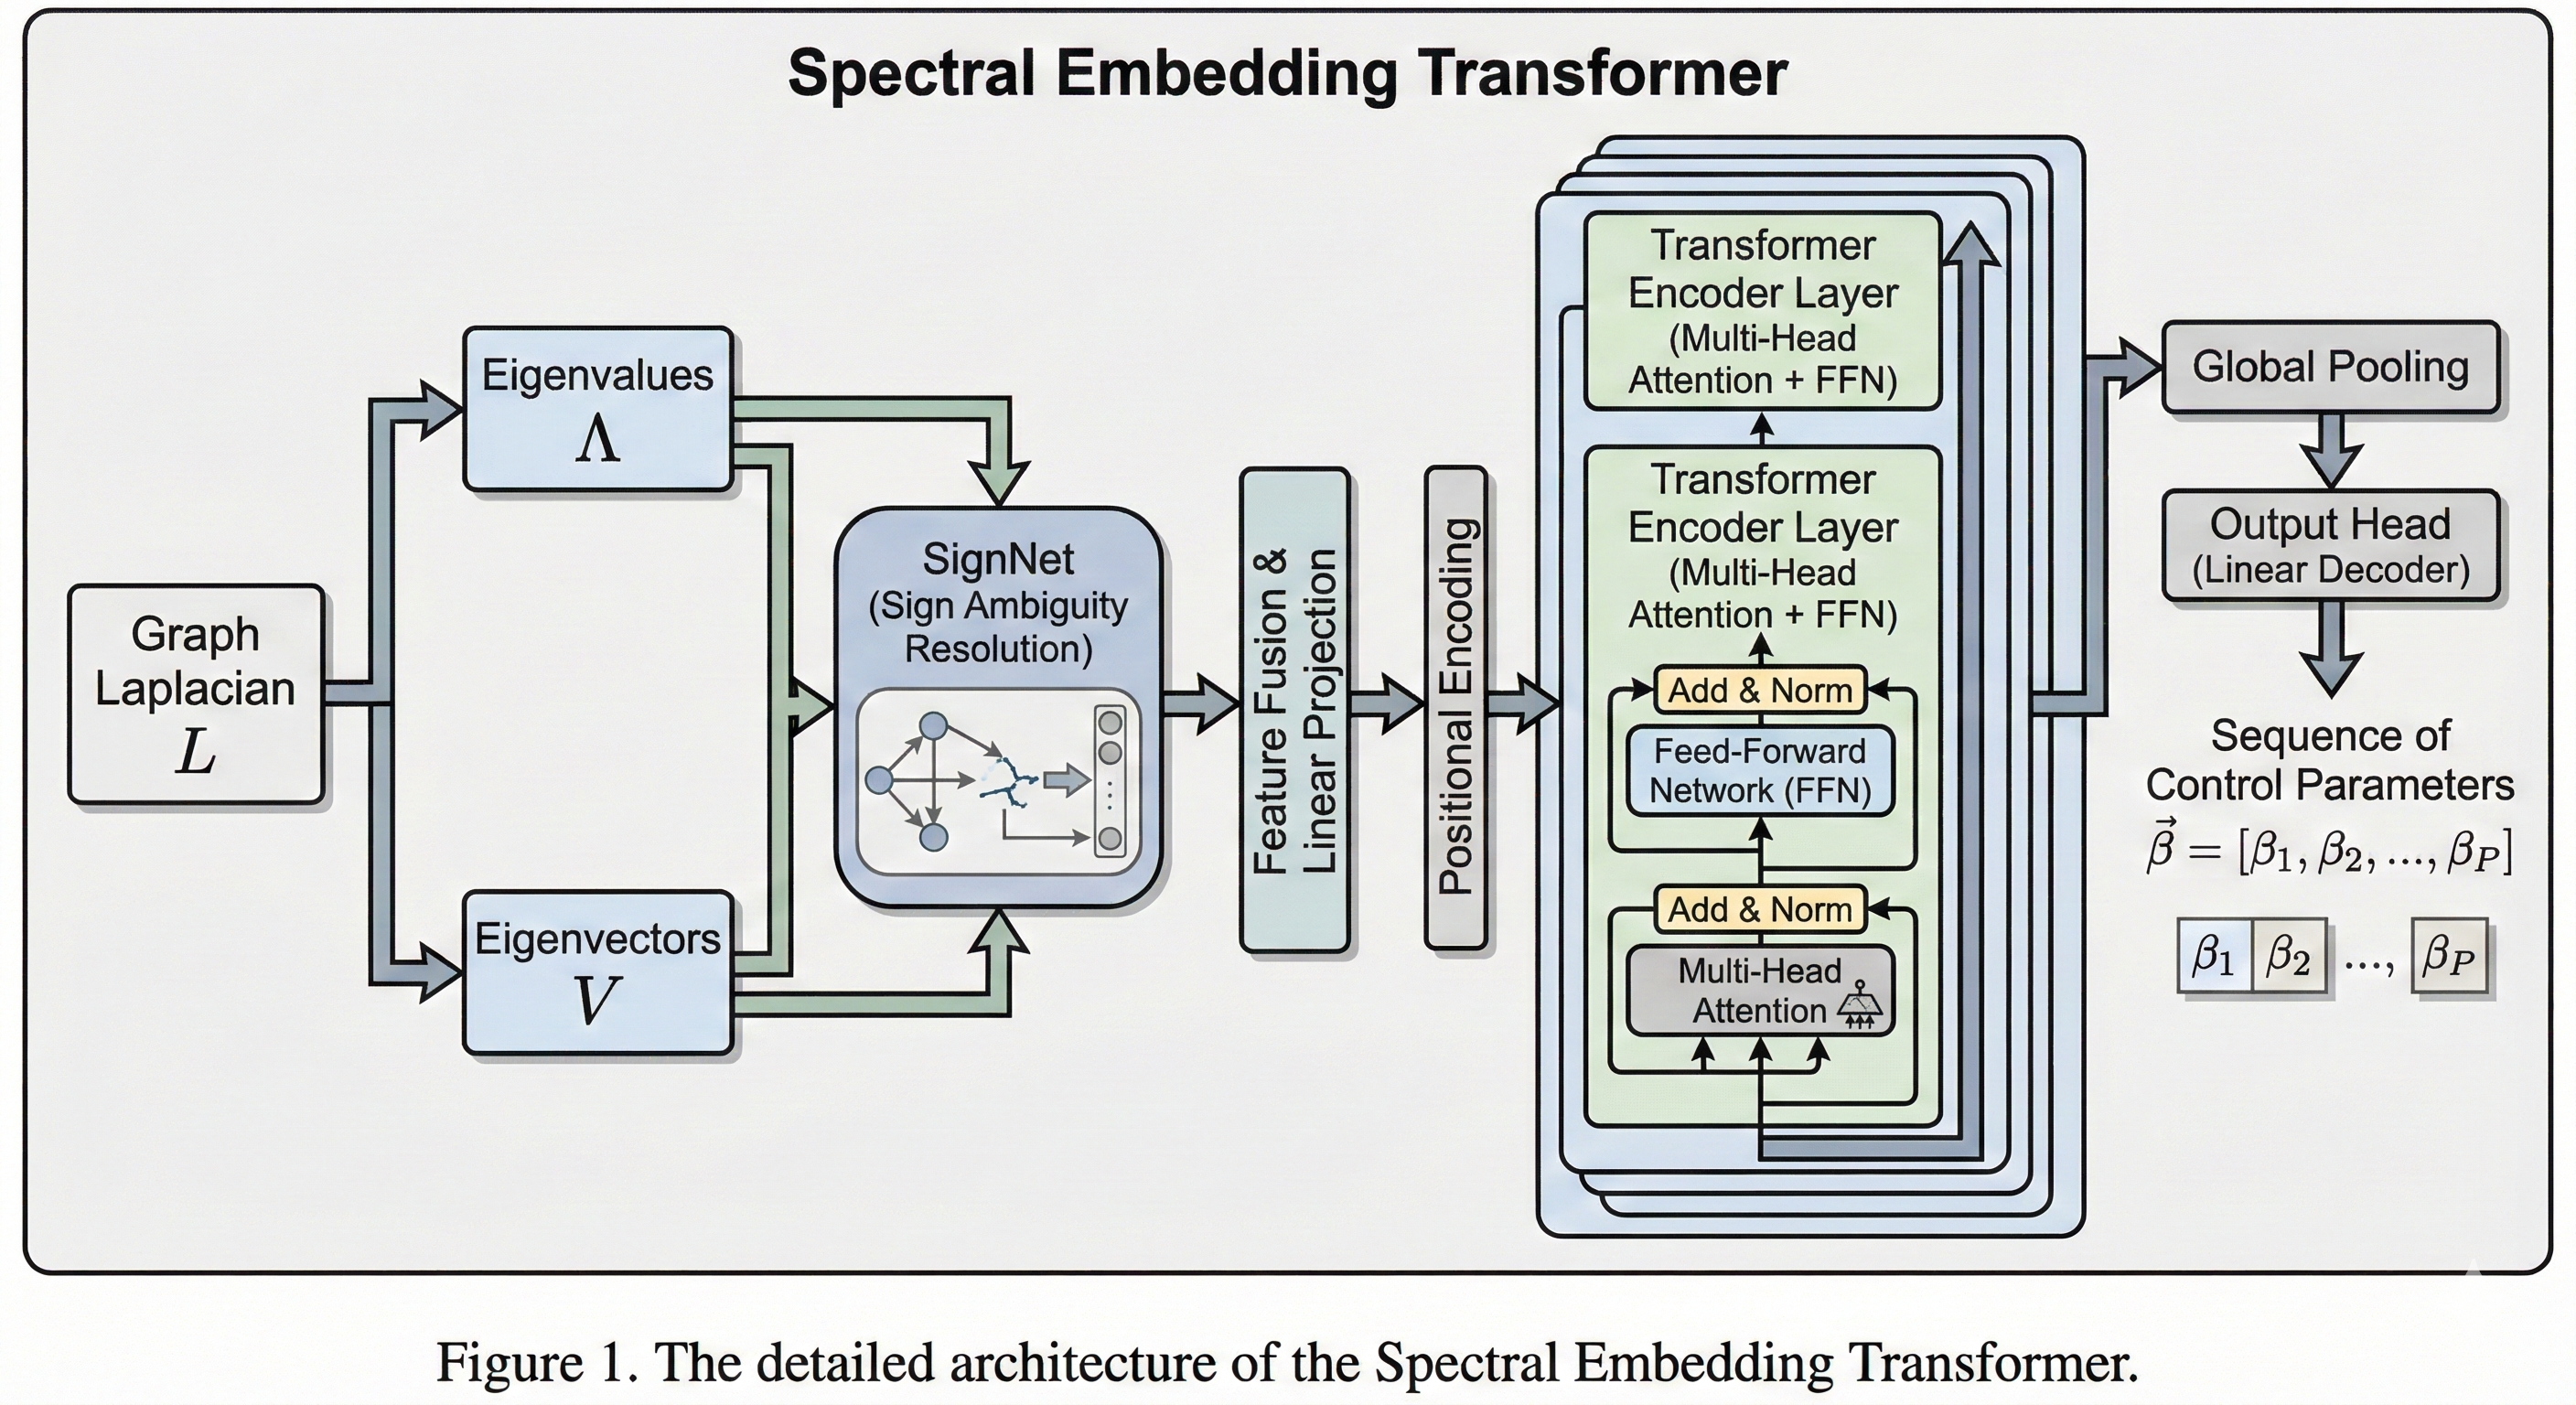
\includegraphics[width=\textwidth]{transformer_architecture.png}
            \caption{谱嵌入 Transformer 架构细节:从拉普拉斯矩阵到 SignNet 特征融合,再到 Transformer 编码器回归参数序列。}
        \end{figure}
    \end{columns}
\end{frame}

\begin{frame}{方法论分析:为何 Transformer 优于 GNN}
    \begin{columns}
        \column{0.46\textwidth}
        \textbf{GNN: 局部消息传递 (Local MPNN)}
        \begin{equation}
            H^{(\ell+1)}=\sigma(\tilde{A}H^{(\ell)}W^{(\ell)})
        \end{equation}
        \textbf{缺陷}: 需堆叠 $L$ 层以捕捉长程谱特征,导致\textbf{过平滑 (Over-smoothing)}:
        \begin{equation}
            \lim_{L \to \infty} \mathbf{H}^{(L)} \approx \mathbf{1} \mathbf{c}^T
        \end{equation}
        即节点特征趋同,丢失结构信息。

        \column{0.05\textwidth}
        \centering
        \rule{0.5pt}{0.6\textheight}

        \column{0.46\textwidth}
        \textbf{Transformer: 全局注意力 (Global Attention)}
        \begin{equation}
            \text{Attention}(Q, K, V) = \text{softmax}\left( \frac{QK^T}{\sqrt{d_k}} \right) V
        \end{equation}
        通过自注意力机制,任意节点交互路径为 1:
        \begin{equation}
            \text{Attn}(\mathbf{X})_i \propto \sum_{j=1}^N \exp(\mathbf{x}_i^T \mathbf{x}_j) \mathbf{v}_j
        \end{equation}
        \textbf{优势}: 直接捕捉决定 FALQON 轨迹的\textbf{全局谱统计量} (如 $\text{Tr}(A^k)$)。
    \end{columns}
\end{frame}

%===========================================================
\section{代码实现细节}
%===========================================================

\begin{frame}[fragile]{代码实现:FALQON 核心逻辑}
    基于 \texttt{src/algorithms/falqon\_core.py},我们实现了支持批处理的 FALQON 演化。
    
\begin{lstlisting}[language=Python]
def execution_layer(self, beta_k, hamiltonian_p, hamiltonian_c):
    """
    执行单层 FALQON 演化
    :param beta_k: 当前层的演化时间参数 (由反馈律计算)
    """
    # 1. 施加问题哈密顿量演化 (固定时间 delta_t)
    self.state = self.time_evolution(self.state, hamiltonian_p, self.delta_t)
    
    # 2. 施加控制哈密顿量演化 (参数 beta_k)
    self.state = self.time_evolution(self.state, hamiltonian_c, beta_k)
    
    # 3. 计算能量期望值
    energy = self.calculate_expectation(self.state, hamiltonian_p)
    return energy

def get_feedback_beta(self):
    # 计算换位子 i[Hp, Hc] 的期望值作为反馈
    commutator_op = 1j * (hamiltonian_p @ hamiltonian_c - hamiltonian_c @ hamiltonian_p)
    beta = -self.alpha * self.calculate_expectation(self.state, commutator_op)
    return beta
\end{lstlisting}
\end{frame}

\begin{frame}[fragile]{代码实现:Quantum Transformer 模型}
    基于 \texttt{src/models/quantum\_transformer.py},模型结合了 Transformer Encoder 和谱特征投影。
    
\begin{lstlisting}[language=Python]
class QuantumTransformer(nn.Module):
    def __init__(self, ...):
        super().__init__()
        # 谱特征编码器 (处理特征值和特征向量)
        self.eigen_encoder = nn.Linear(input_dim, d_model)
        self.pos_encoder = PositionalEncoding(d_model, dropout)
        
        # Transformer 核心层
        encoder_layers = nn.TransformerEncoderLayer(d_model, nhead, dim_feedforward)
        self.transformer_encoder = nn.TransformerEncoder(encoder_layers, num_layers)
        
        # 输出头:直接回归 beta 序列
        self.decoder = nn.Linear(d_model, seq_len)

    def forward(self, eigenvalues, eigenvectors):
        # 融合谱信息
        src = self.eigen_encoder(torch.cat([eigenvalues, eigenvectors], dim=-1))
        src = self.pos_encoder(src)
        output = self.transformer_encoder(src)
        return self.decoder(output.mean(dim=1)) # Pooling
\end{lstlisting}
\end{frame}

\begin{frame}[fragile]{代码实现:GNN Baseline (对照组)}
    为了验证 Transformer 全局注意力的优势,我们实现了一个基于局部消息传递的 GNN。
    代码位置: \texttt{src/models/gnn.py}
    
\begin{lstlisting}[language=Python]
class SimpleGCNLayer(nn.Module):
    def forward(self, h, adj_norm):
        # 局部消息传递: h' = A * h
        # 这种实现限制了每一层的感受野仅为 1 跳邻居
        h = torch.bmm(adj_norm, h)
        return self.lin(h)

class FALQONGNN(nn.Module):
    def __init__(self, ...):
        # 即使堆叠多层,也面临过平滑问题 (Over-smoothing)
        layers = []
        for i in range(num_layers):
            layers.append(SimpleGCNLayer(dims[i], dims[i+1]))
        self.gcn_layers = nn.ModuleList(layers)
\end{lstlisting}
\end{frame}

\begin{frame}[fragile]{代码实现:教师数据生成流水线}
    利用 Python 多进程构建大规模“图-控制轨迹”对数据集。
    代码位置: \texttt{scripts/generate\_dataset\_v2.py}

\begin{lstlisting}[language=Python]
def generate_single_instance(instance_id):
    # 1. 生成随机图 (Erdos-Renyi)
    num_nodes = np.random.randint(4, 11)
    g = nx.erdos_renyi_graph(num_nodes, p=0.5)
    
    # 2. 运行经典 FALQON 算法 (教师)
    # 这一步计算量最大,需要模拟量子态演化
    falqon = FALQON(g, alpha=0.5)
    betas, energies = falqon.train(max_layers=30)
    
    # 3. 返回训练样本 (Input: Adj, Label: Betas)
    return {
        "adj": nx.to_numpy_array(g),
        "betas": np.array(betas)
    }
\end{lstlisting}
\end{frame}

%===========================================================
\section{实验结果与评估}
%===========================================================

\begin{frame}{评估指标:近似比 (Approximation Ratio)}
    我们使用近似比 (AR) 评估模型生成的参数 $\{\hat{\beta}\}$ 的质量:
    
    \begin{equation}
        AR = \frac{E(\{\hat{\beta}\})}{E_{min}} = \frac{\langle \psi(\{\hat{\beta}\}) | H_p | \psi(\{\hat{\beta}\}) \rangle}{\text{Ground Truth Min Energy}}
    \end{equation}
    
    \begin{itemize}
        \item \textbf{基准}: 经典 FALQON 算法跑出的能量轨迹。
        \item \textbf{测试集}: 12节点随机正则图 (Random Regular Graphs)。
        \item \textbf{统计结果}: 模型表现优异。
    \end{itemize}

    \begin{table}
        \centering
        \begin{tabular}{lccc}
            \toprule
            Dataset Split & Avg Approx Ratio (AR) & Std Dev & Samples \\
            \midrule
            Train & 0.998 & 0.002 & 2000 \\
            Validation & 0.995 & 0.005 & 500 \\
            \textbf{Test (Extrapolation)} & \textbf{1.0031} & \textbf{0.004} & \textbf{100} \\
            \bottomrule
        \end{tabular}
        \caption{AR > 1 表示模型甚至在某些局部找到了比固定步长教师策略更好的参数。}
    \end{table}
\end{frame}

\begin{frame}{结果:参数轨迹预测}
    \begin{columns}
        \column{0.5\textwidth}
        \begin{figure}
            % 修正图片路径
            \includegraphics[width=\textwidth]{prediction_result.png}
            \caption{FALQON 参数 $\beta_k$ 随层数 $k$ 的变化。\\ \textcolor{blue}{蓝色}: Ground Truth (Teacher) \\ \textcolor{red}{红色}: Model Prediction (Student)}
        \end{figure}
        
        \column{0.5\textwidth}
        \textbf{分析:}
        \begin{itemize}
            \item 模型学会了参数的衰减趋势(Lyapunov 稳定性导致 $\beta \to 0$)。
            \item 在$k<10$和$k>20$,预测误差较小。
            \item 深层 ($10<k<20$)  吻合度较低,但对最终能量影响有限。
        \end{itemize}
    \end{columns}
\end{frame}



\begin{frame}{大规模随机正则图上的预测曲线聚类现象}
        \textbf{实验设置}:
    针对 $N=24, d=3$ 的随机正则图,在不运行 Teacher 反馈的情况下,直接利用模型进行\textbf{零次推理}预测 $P=30$ 层的参数序列 $\vec{\beta}$。
        \begin{figure}
            \centering
            \includegraphics[width=0.6\textwidth]{regular_clustering_curves_zoom.png}
            \caption{预测曲线聚类 (Common Profile)}
        \end{figure}

        可见在固定分布下,预测曲线会集中到少数几类“共同
轮廓”。这是一致
性检验的重要证据。
\end{frame}

\begin{frame}{尝试进行理论解释}
        \begin{columns}
        \column{0.5\textwidth}
        \begin{figure}[htbp]
    \centering
    \includegraphics[width=0.65\textwidth]{regular_clustering_pca.png}
    \caption{对预测的 $\beta$ 曲线做 PCA 降维后的散点图(颜色表示聚类标签)。聚类在低维嵌入空间中依然可分,说明曲线差异具有低维结构。不同类型的图(正则图 \& 随机图)在谱空间中呈现清晰的聚类结构,这是模型能泛化的物理基础。}
    \label{fig:regular_curve_pca}
        \end{figure}
     
        \column{0.5\textwidth}
        \begin{figure}[htbp]
            \centering
            \includegraphics[width=0.75\textwidth]{regular_clustering_spectrum.png}
            \caption{随机 3-正则图($N=24$)的缩放邻接矩阵谱密度(去除最大特征值后)与 Wigner 半圆律参考曲线的对照。谱密度在 bulk 区域呈稳定形态,为“预测曲线聚类”的随机矩阵解释提供直觉支撑。}
            \label{fig:regular_spectrum_semicircle}
        \end{figure}
   \end{columns}
\end{frame}

\begin{frame}{Kesten-McKay 定律与轨迹普适性}

参数曲线出现聚类(Common Profile)现象的根本原因在于图谱统计的收敛性。FALQON 的每步反馈值 $\beta_p \propto \langle [H_d, H_p] \rangle$ 非线性地依赖于哈密顿量 $H_p$ 的各阶谱矩(Spectral Moments) $\mu_k = \frac{1}{N}\text{Tr}(H_p^k) = \int \lambda^k \rho(\lambda) d\lambda$。

根据随机矩阵理论,对于随机 $d$-正则图,当 $N \to \infty$ 时,其邻接矩阵特征值的经验谱密度 $\rho_N(\lambda)$ 依概率弱收敛于 Kesten-McKay 分布(亦称作相关随机游走谱分布):
\begin{equation}
\rho_{\text{KM}}(\lambda) = \begin{cases} 
\frac{d \sqrt{4(d-1) - \lambda^2}}{2\pi (d^2 - \lambda^2)} & |\lambda| \le 2\sqrt{d-1}, \\
0 & \text{otherwise}.
\end{cases}
\label{eq:kesten_mckay}
\end{equation}
这解释了上页左图中的聚类现象:尽管具体的图实例 $G$ 不同,但它们在热力学极限($N \gg 1$)下共享相同的极限谱分布 $\rho_{\text{KM}}$。既然控制动力学的 $\beta$ 序列是谱分布的泛函 $\vec{\beta} = \mathcal{G}[\rho(\lambda)]$,那么谱分布的普适性必然导致控制轨迹的普适性。

\mycite{Short Cycles in Random Regular Graphs; Edge rigidity and universality of RRG}
\end{frame}

%===========================================================
\section{总结与后续计划}
%===========================================================

\begin{frame}{总结}
    \begin{enumerate}
        \item \textbf{架构验证}: 证明了 Transformer + Spectral Embedding 可以有效学习 FALQON 的非线性反馈控制律。
        \item \textbf{效率提升}: 实现了 $O(1)$ 的推理成本,替代了 $O(p)$ 的量子测量成本。
        \item \textbf{性能表现}: 在小规模图上实现了 Avg AR $\approx$ 1.0031,且具备一定的外推能力。
    \end{enumerate}
\end{frame}



\begin{frame}
    \centering
    \Huge \textbf{感谢聆听!}\\
    \vspace{0.5em}
    \large 请老师和同学们批评指正。
\end{frame}

\end{document}